\chapter*{IDENTASI}

\section*{Penjelasan, membaca error dan menangani Identasi}

\par
Identasi merupakan salah satu bagian paragraf yang menjorok kedalam pada baris didalam paragraf, tidak menggunakan curly brackets "{}" untuk membedakan bagian program digunakan identasi. untuk mengetahui jenis errornya dapat diketahui melalui IndentitionError: expected an idented block. untuk menghindari error ini bisa menggunakan fungsi if memerlukan identasi untuk membedakannya.

\begin{figure} [h]
	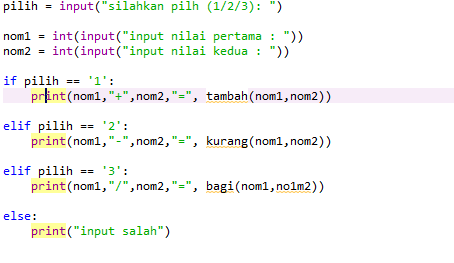
\includegraphics[width=12cm]{section/spy/li.png}
	\centering
	\end{figure}
	
	
	
